% THIS DOCUMENT IS TAILORED TO REQUIREMENTS FOR SCIENTIFIC COMPUTING.  IT SHOULDN'T BE USED FOR
% NON-SCIENTIFIC COMPUTING PROJECTS
\documentclass[12pt]{article}

\usepackage{amsmath, mathtools}
\usepackage{amsfonts}
\usepackage{amssymb}
\usepackage{bm}
\usepackage{graphicx}
\usepackage{colortbl}
\usepackage{xr}
\usepackage{hyperref}
\usepackage{longtable}
\usepackage{xfrac}
\usepackage{tabularx}
\usepackage{float}
\usepackage{siunitx}
\usepackage{booktabs}
\usepackage{caption}
\usepackage{pdflscape}
\usepackage{afterpage}
\usepackage{cite}
% \usepackage[round]{natbib} \usepackage{refcheck}

\hypersetup{ bookmarks=true,       % show bookmarks bar?
    colorlinks=true,      % false: boxed links; true: colored links
    linkcolor=red,          % color of internal links (change box color with linkbordercolor)
    citecolor=green,        % color of links to bibliography
    filecolor=magenta,      % color of file links
    urlcolor=cyan           % color of external links
}

%% Comments

\usepackage{color}

% \newif\ifcomments\commentstrue %displays comments
\newif\ifcomments\commentsfalse %so that comments do not display

\ifcomments
\newcommand{\authornote}[3]{\textcolor{#1}{[#3 ---#2]}}
\newcommand{\todo}[1]{\textcolor{red}{[TODO: #1]}}
\else
\newcommand{\authornote}[3]{}
\newcommand{\todo}[1]{}
\fi

\newcommand{\wss}[1]{\authornote{blue}{SS}{#1}} 
\newcommand{\plt}[1]{\authornote{magenta}{TPLT}{#1}} %For explanation of the template
\newcommand{\an}[1]{\authornote{cyan}{Author}{#1}}

%% Common Parts

\newcommand{\progname}{ProgName} % PUT YOUR PROGRAM NAME HERE
\newcommand{\authname}{Adrian Sochaniwsky} % AUTHOR NAMES                  

\usepackage{hyperref}
    \hypersetup{colorlinks=true, linkcolor=blue, citecolor=blue, filecolor=blue,
                urlcolor=blue, unicode=false}
    \urlstyle{same}
                                


% For easy change of table widths
\newcommand{\colZwidth}{1.0\textwidth}
\newcommand{\colAwidth}{0.13\textwidth}
\newcommand{\colBwidth}{0.82\textwidth}
\newcommand{\colCwidth}{0.1\textwidth}
\newcommand{\colDwidth}{0.05\textwidth}
\newcommand{\colEwidth}{0.8\textwidth}
\newcommand{\colFwidth}{0.17\textwidth}
\newcommand{\colGwidth}{0.5\textwidth}
\newcommand{\colHwidth}{0.28\textwidth}

% Used so that cross-references have a meaningful prefix
\newcounter{defnum} %Definition Number
\newcommand{\dthedefnum}{GD\thedefnum}
\newcommand{\dref}[1]{GD\ref{#1}} \newcounter{datadefnum} %Datadefinition Number
\newcommand{\ddthedatadefnum}{DD\thedatadefnum}
\newcommand{\ddref}[1]{DD\ref{#1}} \newcounter{theorynum} %Theory Number
\newcommand{\tthetheorynum}{TM\thetheorynum}
\newcommand{\tref}[1]{TM\ref{#1}} \newcounter{tablenum} %Table Number
\newcommand{\tbthetablenum}{TB\thetablenum}
\newcommand{\tbref}[1]{TB\ref{#1}} \newcounter{assumpnum} %Assumption Number
\newcommand{\atheassumpnum}{A\theassumpnum}
\newcommand{\aref}[1]{A\ref{#1}} \newcounter{goalnum} %Goal Number
\newcommand{\gthegoalnum}{GS\thegoalnum}
\newcommand{\gsref}[1]{GS\ref{#1}} \newcounter{instnum} %Instance Number
\newcommand{\itheinstnum}{IM\theinstnum}
\newcommand{\iref}[1]{IM\ref{#1}} \newcounter{reqnum} %Requirement Number
\newcommand{\rthereqnum}{R\thereqnum}
\newcommand{\rref}[1]{R\ref{#1}} \newcounter{nfrnum} %NFR Number
\newcommand{\rthenfrnum}{NFR\thenfrnum}
\newcommand{\nfrref}[1]{NFR\ref{#1}} \newcounter{lcnum} %Likely change number
\newcommand{\lthelcnum}{LC\thelcnum}
\newcommand{\lcref}[1]{LC\ref{#1}}

\usepackage{fullpage}

\newcommand{\deftheory}[9][Not Applicable]
{
\newpage
\noindent \rule{\textwidth}{0.5mm}

\paragraph{RefName: } \refstepcounter{theorynum}\tthetheorynum 
\label{#2}
\paragraph{Label:} #3

\noindent \rule{\textwidth}{0.5mm}

\paragraph{Equation:}

#4

\paragraph{Description:}

#5

\paragraph{Notes:}

#6

\paragraph{Source:}

#7

\paragraph{Ref.\ By:}

#8

\paragraph{Preconditions for \tref{#2}:}
\label{#2_precond}

#9

\paragraph{Derivation for \tref{#2}:}
\label{#2_deriv}

#1

\noindent \rule{\textwidth}{0.5mm}

}

\begin{document}

\title{Software Requirements Specification for Attitude Check: IMU-based Attitude Estimation} 
\author{\authname}
\date{\today}
	
\maketitle

~\newpage

\pagenumbering{roman}

\tableofcontents

~\newpage

\section*{Revision History}

\begin{tabularx}{\textwidth}{p{3cm}p{2cm}X} \toprule {\bf Date} & {\bf Version} & {\bf Notes}\\
\midrule
2024/02/02 & 1.0 & Initial Release.\\
\bottomrule
\end{tabularx}

~\newpage

\section{Reference Material}

This section records information for easy reference.

\subsection{Table of Units}

Throughout this document SI (Syst\`{e}me International d'Unit\'{e}s) is employed as the unit system.
In addition to the basic units, several derived units are used as described below.  For each unit,
the symbol is given followed by a description of the unit and the SI name. ~\newline

\renewcommand{\arraystretch}{1.2}
%\begin{table}[ht]
  \noindent \begin{tabular}{l l l} 
    \toprule		
    \textbf{symbol} & \textbf{unit} & \textbf{SI}\\
    \midrule 
    \si{\metre} & length & metre\\
    \si{\radian} & angle & radian\\
    \si{\second} & time & second\\
    % \si{\hertz} & frequency & hertz\\
    \si{\tesla}      & magnetic field & tesla \\
    % \si{\kilogram} & mass & kilogram\\
    \bottomrule
  \end{tabular}
  %	\caption{Provide a caption}
%\end{table}

\plt{Only include the units that your SRS actually uses.}

\plt{Derived units, like newtons, pascal, etc, should show their derivation (the units they are
    derived from) if their constituent units are in the table of units (that is, if the units they
    are derived from are used in the document).  For instance, the derivation of pascals as
    $\si{\pascal}=\si{\newton\per\square\meter}$ is shown if newtons and m are both in the table.
    The derivations of newtons would not be shown if kg and s are not both in the table.}

\plt{The symbol for units named after people use capital letters, but the name of the unit itself
  uses lower case.  For instance, pascals use the symbol Pa, watts use the symbol W, teslas use the
  symbol T, newtons use the symbol N, etc.  The one exception to this is degree Celsius.  Details on
  writing metric units can be found on the 
  \href{https://www.nist.gov/pml/weights-and-measures/writing-metric-units}
  {NIST} web-page.}

\subsection{Table of Symbols}

The table that follows summarizes the symbols used in this document along with their units.  The
choice of symbols was made to be consistent with the attitude and heading reference systems
literature and existing documentation. The symbols are listed in alphabetical order.

\renewcommand{\arraystretch}{1.2}
%\noindent \begin{tabularx}{1.0\textwidth}{l l X}
\noindent \begin{longtable*}{l l p{12cm}} \toprule \textbf{symbol} & \textbf{unit} &
\textbf{description}\\
\midrule 
% $v$ & \si[per-mode=symbol] {\meter\per\second} & linear velocity\\
$a$ & \si[per-mode=symbol] {\meter\per\second\squared} & linear acceleration\\
$m$ & \si[per-mode=symbol] {\tesla} & magnetic field strength\\
$\theta$ & \si[per-mode=symbol] {\radian} & angular position \\
$\omega$ & \si[per-mode=symbol] {\radian\per\second} & angular velocity\\
$\Delta t$ & \si[per-mode=symbol] {\milli\second} & sampling time\\
$\mathbf{g}_0$ & \si[per-mode=symbol] {\meter\per\second\squared} & gravitational acceleration
vector\\
${}^E\mathbf{b}$ & \si{\nano\tesla} & local magnetic field vector\\
$\gamma$ & - & Complimentary filter parameter\\
${}^S_E\mathbf{q}$ & \si{\radian} & Attitude (orientation) of the sensor-frame relative to the
earth-frame\\
$\eta$ & - & Fraction of development time\\
\bottomrule
\end{longtable*}
\plt{Use your problems actual symbols.  The si package is a good idea to use for units.}

\subsection{Abbreviations and Acronyms}

\renewcommand{\arraystretch}{1.2}
\begin{tabular}{l l} 
  \toprule		
  \textbf{symbol} & \textbf{description}\\
  \midrule 
  A & Assumption\\
  API & Application Programming Interface \\
  DD & Data Definition\\
  GD & General Definition\\
  GS & Goal Statement\\
  IM & Instance Model\\
  LC & Likely Change\\
  PS & Physical System Description\\
  R & Requirement\\
  SRS & Software Requirements Specification\\
  % \progname{} & \plt{put an expanded version of your program name here (as appropriate)}\\
  TM & Theoretical Model\\
  IMU & Inertial Measurement Unit\\
  MEMS & Micro-electromechanical System \\
  NED & North-East-Down \\
  WMM & World Magnetic Model. \\
  \bottomrule
\end{tabular}\\

\plt{Add any other abbreviations or acronyms that you add}

\subsection{Mathematical Notation}

\begin{itemize}
  \item[Vector:] Vectors will be distinguished via \textbf{bold} face font such as, $\mathbf{b}$.
  \item[Matrix:] Matrices will be distinguished via \textbf{bold} face font and capitalization such
  as, $\mathbf{R}$.
  \item[Time:] Variables for a given time step, $t$ will be denoted with a sub-postscript such as,
  $\mathbf{s}_t$.
  \item[Frame:] The reference frame for a variable will be denoted by a super-prescript, such as
  $\prescript{E}{}{\mathbf{s}}$. Where the vector $\mathbf{s}$ taken with respect to the Earth
  frame.
  \item[Transform:] The rotational transform between two frames will be denoted using pre-scripts.
  For example, $\prescript{B}{A}{\mathbf{T}}$ describes the orientation of frame A relative to B.
\end{itemize}

\plt{This section is optional, but should be included for projects that make use of notation to
  convey mathematical information.  For instance, if typographic conventions (like bold face font)
  are used to distinguish matrices, this should be stated here.  If symbols are used to show
  mathematical operations, these should be summarized here.  In some cases the easiest way to
  summarize the notation is to point to a text or other source that explains the notation.}

\plt{This section was added to the template because some students use very domain specific notation.
  This notation will not be readily understandable to people outside of your domain.  It should be
  explained.}

\newpage

\pagenumbering{arabic}

\plt{This SRS template is based on \cite{SmithAndLai2005, SmithEtAl2007, SmithAndKoothoor2016}.  It
  will get you started.  You should not modify the section headings, without first discussing the
  change with the course instructor.  Modification means you are not following the template, which
  loses some of the advantage of a template, especially standardization. Although the bits shown
  below do not include type information, you may need to add this information for your problem.  If
  you are unsure, please can ask the instructor.}

\plt{Feel free to change the appearance of the report by modifying the LaTeX commands.}

\plt{This template document assumes that a single program is being documented. If you are
  documenting a family of models, you should start with a commonality analysis.  A separate template
  is provided for this.  For program families you should look at \cite{Smith2006,
  SmithMcCutchanAndCarette2017}. Single family member programs are often programs based on a single
  physical model.  General purpose tools are usually documented as a family.  Families of physical
  models also come up.}

\plt{The SRS is not generally written, or read, sequentially.  The SRS is a reference document.  It
  is generally read in an ad hoc order, as the need arises.  For writing an SRS, and for reading one
  for the first time, the suggested order of sections is:
\begin{itemize}
\item Goal Statement
\item Instance Models
\item Requirements
\item Introduction
\item Specific System Description
\end{itemize}
}

\plt{Guiding principles for the SRS document:
\begin{itemize}
\item Do not repeat the same information at the same abstraction level.  If information is repeated,
  the repetition should be at a different abstraction level.  For instance, there will be overlap
  between the scope section and the assumptions, but the scope section will not go into as much
  detail as the assumptions section.
\end{itemize}
}

\plt{The template description comments should be disabled before submitting this document for
  grading.}

\plt{You can borrow any wording from the text given in the template.  It is part of the template,
  and not considered an instance of academic integrity.  Of course, you need to cite the source of
  the template.}

\plt{When the documentation is done, it should be possible to trace back to the source of every
  piece of information.  Some information will come from external sources, like terminology.  Other
  information will be derived, like General Definitions.}

\plt{An SRS document should have the following qualities: unambiguous, consistent, complete,
  validatable, abstract and traceable.}

\plt{The overall goal of the SRS is that someone that meets the Characteristics of the Intended
  Reader (Section~\ref{sec_IntendedReader}) can learn, understand and verify the captured domain
  knowledge.  They should not have to trust the authors of the SRS on any statements.  They should
  be able to independently verify/derive every statement made.}

\section{Introduction}

The goal of attitude estimation is to determine the rotation of an object relative to a reference
frame using sensor measurements. Attitude estimation is essential for many applications, such as
navigation and control of spacecraft, drones, or robots. Once only possible with expensive hardware,
advances in Micro-Electro-Mechanical systems (MEMS) allow an inexpensive Inertial Measurement Unit
(IMU) to provide the necessary measurements for attitude estimation. Typical IMU sensors contain a
3-axis accelerometer, 3-axis magnetometer, and 3-axis gyroscope. However, challenges arise from the
presence of noise, bias, drift, and uncertainty in the sensor data, as well as the nonlinearity of
the object dynamics \cite{statement}.

\plt{The introduction section is written to introduce the problem.  It starts general and focuses on
  the problem domain. The general advice is to start with a paragraph or two that describes the
  problem, followed by a ``roadmap'' paragraph.  A roadmap orients the reader by telling them what
  sub-sections to expect in the Introduction section.}


\subsection{Purpose of Document}

\plt{This section summarizes the purpose of the SRS document.  It does not focus on the problem
  itself.  The problem is described in the ``Problem Description'' section (Section~\ref{Sec_pd}).
  The purpose is for the document in the context of the project itself, not in the context of this
  course. Although the ``purpose'' of the document is to get a grade, you should not mention this.
  Instead, ``fake it'' as if this is a real project.  The purpose section will be similar between
  projects.  The purpose of the document is the purpose of the SRS, including communication,
  planning for the design stage, etc.}

This document defines the scope, requirements, and functionality, of a software product. It serves
as a contract between the developers and the stakeholders, ensuring that both parties have a clear
and common understanding of what the software should do and how it should perform. This SRS also
helps the developers to plan, design, test, and maintain the software according to the agreed-upon
requirements. This document can reduce the risk of errors, delays, and conflicts during the software
development process. \cite{purpose}

\subsection{Scope of Requirements}

The scope of this document will only consider operating conditions where all measured values are
within the range of the sensors, and the system is at or near the surface of the Earth.

Furthermore, time varying changes in the Earths magnetic field are ignored.

\plt{Modelling the real world requires simplification.  The full complexity of the actual physics,
  chemistry, biology is too much for existing models, and for existing computational solution
  techniques.  Rather than say what is in the scope, it is usually easier to say what is not.  You
  can think of it as the scope is initially everything, and then it is constrained to create the
  actual scope.  For instance, the problem can be restricted to 2 dimensions, or it can ignore the
  effect of temperature (or pressure) on the material properties, etc.}  

\plt{The scope section is related to the assumptions section (Section~\ref{sec_assumpt}).  However,
  the scope and the assumptions are not at the same level of abstraction.  The scope is at a high
  level.  The focus is on the ``big picture'' assumptions.  The assumptions section lists, and
  describes, all of the assumptions.}

\subsection{Characteristics of Intended Reader} \label{sec_IntendedReader}

The reader should have a university-level understanding of matrix and vector operations, numerical
methods, state estimation, and dynamics. The reader should have some familiarity with digital
sensors.

\plt{This section summarizes the skills and knowledge of the readers of the SRS.  It does NOT have
  the same purpose as the ``User Characteristics'' section (Section~\ref{SecUserCharacteristics}).
  The intended readers are the people that will read, review and maintain the SRS.  They are the
  people that will conceivably design the software that is intended to meet the requirements.  The
  user, on the other hand, is the person that uses the software that is built.  They may never read
  this SRS document.  Of course, the same person could be a ``user'' and an ``intended reader.''}

\plt{The intended reader characteristics should be written as unambiguously and as specifically as
  possible.  Rather than say, the user should have an understanding of physics, say what kind of
  physics and at what level.  For instance, is high school physics adequate, or should the reader
  have had a graduate course on advanced quantum mechanics?}

\subsection{Organization of Document}

The rest of this document is structured as follows. Section \ref{sec:general_desc} discusses the
general context and description of the system. Section \ref{sec:specific_user_desc} details the
specific system description, goals, and definitions. Section \ref{sec:reqs} covers system
requirements. Section \ref{sec:likely_changes} outlines likely changes for the system. Section
\ref{sec:unlikely_changes} discusses unlikely changes. Section \ref{sec:trace} covers the
traceability of the requirements. Section \ref{sec:dev_plan} discusses the system development plan.

\plt{This section provides a roadmap of the SRS document.  It will help the reader orient
  themselves.  It will provide direction that will help them select which sections they want to
  read, and in what order.  This section will be similar between project.}

\section{General System Description} \label{sec:general_desc}

This section provides general information about the system.  It identifies the interfaces between
the system and its environment, describes the user characteristics and lists the system constraints.
\plt{This text can likely be borrowed verbatim.}

\plt{The purpose of this section is to provide general information about the system so the specific
  requirements in the next section will be easier to understand. The general system description
  section is designed to be changeable independent of changes to the functional requirements
  documented in the specific system description. The general system description provides a context
  for a family of related models.  The general description can stay the same, while specific details
  are changed between family members.}

\subsection{System Context}

\plt{Your system context will include a figure that shows the abstract view of the software.  Often
  in a scientific context, the program can be viewed abstractly following the design pattern of
  Inputs $\rightarrow$ Calculations $\rightarrow$ Outputs.  The system context will therefore often
  follow this pattern.  The user provides inputs, the system does the calculations, and then
  provides the outputs to the user.  The figure should not show all of the inputs, just an abstract
  view of the main categories of inputs (like material properties, geometry, etc.).  Likewise, the
  outputs should be presented from an abstract point of view.  In some cases the diagram will show
  other external entities, besides the user.  For instance, when the software product is a library,
  the user will be another software program, not an actual end user. If there are system constraints
  that the software must work with external libraries, these libraries can also be shown on the
  System Context diagram. They should only be named with a specific library name if this is required
  by the system constraint.}

Attitude estimation is a lower-level operation in an overall robotics or aerospace application. Once
the hardware is installed and the software is compiled, there is no direct human interaction with
the system in the context of measuring or estimating orientation. Figure \ref{fig:systemContext}
shows the general system context of Attitude Check, the IMU measurements are filtered and the
orientation estimate is calculated for downstream use. Higher level functions that perform guidance,
navigation, and control consume orientation to complete higher level objectives.

\begin{figure}[h!]
    \centerline{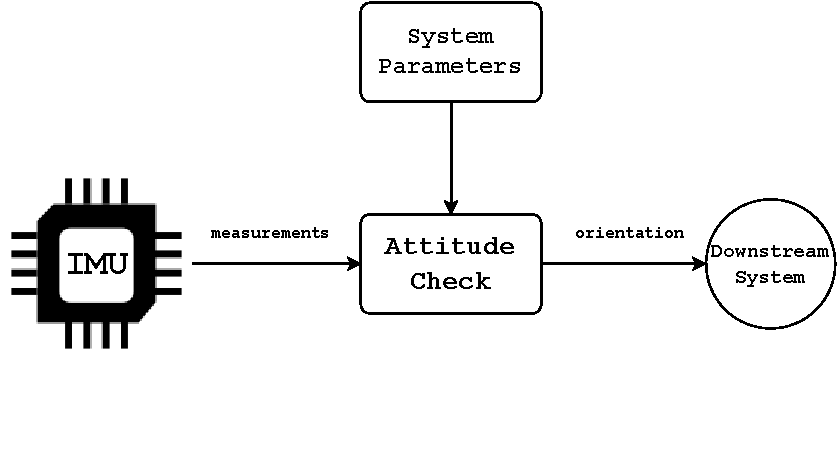
\includegraphics[width=0.6\textwidth, trim={0 2cm 0
    0},clip]{cas741_attitudeCheck.pdf}}
    \caption{System Context}
    \label{fig:systemContext} 
\end{figure}

\plt{For each of the entities in the system context diagram its responsibilities should be listed.
    Whenever possible the system should check for data quality, but for some cases the user will
    need to assume that responsibility.  The list of responsibilites should be about the inputs and
    outputs only, and they should be abstract.  Details should not be presented here.  However, the
    information should not be so abstract as to just say ``inputs'' and ``outputs''.  A summarizing
    phrase can be used to characterize the inputs. For instance, saying ``material properties''
    provides some information, but it stays away from the detail of listing every required
    properties.}

\begin{itemize}
    \item User Responsibilities:
\begin{itemize}
    \item Provide IMU measurements.
    \item Provide a gain value for the filter.
\end{itemize}
    \item \progname{} Responsibilities:
\begin{itemize}
    \item Detect data type mismatch, such as a string of characters instead of a floating point
  number.
    \item Return orientation value for each set of measurements.
\end{itemize}
\end{itemize}

\subsection{User Characteristics} \label{SecUserCharacteristics}

The typical user of \progname{} is expected to have an understanding of the purpose, inputs, and
output of an attitude estimator. This project is designed for users looking to process IMU data.
High-school level kinematics is required. For optimal results the user will be required to adjust
the gain parameter, this may require experimentation. 

\plt{This section summarizes the knowledge/skills expected of the user. Measuring usability, which
  is often a required non-function requirement, requires knowledge of a typical user.  As mentioned
  above, the user is a different role from the ``intended reader,'' as given in
  Section~\ref{sec_IntendedReader}.  As in Section~\ref{sec_IntendedReader}, the user
  characteristics should be specific an unambiguous.  For instance, ``The end user of \progname{}
  should have an understanding of undergraduate Level 1 Calculus and Physics.''}

\subsection{System Constraints}

Attitude Check is often ported to microcontrollers or used in high performance applications. Since
existing infrastructure for system that require attitude estimation are developed in C/C++, this
library should use the same programming language for ease of integration. 

\plt{System constraints differ from other type of requirements because they limit the developers'
  options in the system design and they identify how the eventual system must fit into the world.
  This is the only place in the SRS where design decisions can be specified.  That is, the quality
  requirement for abstraction is relaxed here.  However, system constraints should only be included
  if they are truly required.}

\section{Specific System Description} \label{sec:specific_user_desc}

This section first presents the problem description, which gives a high-level view of the problem to
be solved.  This is followed by the solution characteristics specification, which presents the
assumptions, theories, definitions and finally the instance models.  \plt{Add any project specific
details that are relevant for the section overview.}

\subsection{Problem Description} \label{Sec_pd}

\progname{} is intended to estimate the attitude of an IMU sensor, given noisy measurements.

\plt{What problem does your program solve? The description here should be in the problem space, not
the solution space.}

\subsubsection{Terminology and  Definitions}

\plt{This section is expressed in words, not with equations.  It provide the meaning of the
  different words and phrases used in the domain of the problem. The terminology is used to
  introduce concepts from the world outside of the mathematical model  The terminology provides a
  real world connection to give the mathematical model meaning.}

This subsection provides a list of terms that are used in the subsequent sections and their meaning,
with the purpose of reducing ambiguity and making it easier to correctly understand the
requirements:

\begin{itemize}

\item Attitude: Also referred to as orientation, is the angle of an object relative to another frame
of reference
\item Coordinate frame: the 3D frame of reference for a particular rigid body, comprised of 3
orthogonal vectors that follow the right-hand rule.
\item Euler angles: An intuitive method of representing rotations in 3D space, Euler angles use 3
rotations about the x, y, and z axes. This representation is susceptible to gimbal lock, when 2 axes
are parallel, the 3rd axis is immobile.
\item Requirement: A statement of a functional or non-functional property that a software system
should accomplish.
\item Rotation Matrix: a $n \times n$ matrix used to perform rotation transformations in Euclidean
space. They are also used to describe the orientation of a rigid body.
\item Transform: a computation that converts data from one coordinate frame to another.
\item Quaternion: A quaternion is a compact mathematical notation for representing 3D rotations.
Unlike Euler angles, quaternions are not subject to gimbal lock. See \cite{quat} for more
information.
\end{itemize}

\subsubsection{Physical System Description} \label{sec_phySystDescrip}

\plt{The purpose of this section is to clearly and unambiguously state the physical system that is
  to be modelled. Effective problem solving requires a logical and organized approach. The
  statements on the physical system to be studied should cover enough information to solve the
  problem. The physical description involves element identification, where elements are defined as
  independent and separable items of the physical system. Some example elements include acceleration
  due to gravity, the mass of an object, and the size and shape of an object. Each element should be
  identified and labelled, with their interesting properties specified clearly. The physical
  description can also include interactions of the elements, such as the following: i) the
  interactions between the elements and their physical environment; ii) the interactions between
  elements; and, iii) the initial or boundary conditions.}

The physical system of \progname{}, as shown in Figure \ref{fig:ref_diag} includes the following
elements:

\begin{itemize}
  \item[\textbf{PS1:}] Problem Domain is $\mathbb{R}^3$.

  \item[\textbf{PS2:}] Coordinate Frames:
  \begin{itemize}
      \item[\textbf{PS2a}] Sensor frame: This is a non-inertial reference frame that aligns with the
      IMU output \cite{al-jlailaty_efficient_2020}. Figure \ref{fig:ref_diag} shows the details:
        \begin{itemize}
            \item The origin is at the mass center of the IMU.
            \item The x-axis points to the front of the IMU.
            \item The y-axis points to the right of the IMU.
            \item The z-axis points down, perpendicular to the x-y plane.
        \end{itemize}
    \item[\textbf{PS2b}] Navigation Frame: This is a reference frame used to describe the IMU
    orientation relative to the earth surface, shown in Figure \ref{fig:ref_diag} as the n-frame.
    The origin is below the mass center of the IMU, on the Earths surface, the axes follow the
    North-East-Down (NED) convention, see \cite{ned} for details.

    \item[\textbf{PS2c}] Earth Frame: This is a coordinate system attached to the Earth. Also
    referred to as the e-frame, it is defined by:
    \begin{itemize}
        \item The origin is at the mass center of the Earth.
        \item The x-axis points to the Greenwich meridian.
        \item The y-axis is 90 degrees of the Greenwich meridian.
        \item The z-axis is the rotational axis of the Earth.
        \end{itemize}
  \end{itemize}
  
  \item[\textbf{PS3:}] Forces:
  \begin{itemize}
    \item[\textbf{PS3a:}] Gravitational Force. All objects in the domain that have mass are subject
    to gravitational acceleration that is perpendicular to the surface of the earth. This force may
    vary with position on the Earth's surface.
    \item[\textbf{PS3b:}] Magnetic Force. The strength of the Earth's magnetic field can be measured
    to assist attitude estimation \cite{magnet}. It may vary with position on the Earth's surface or
    time.
  \end{itemize}
  \item[\textbf{PS4:}] Initial conditions. The initial condition is the orientation of the system at
  startup. It is an optional value provided by the user. Otherwise, the system will produce an
  estimated initial orientation.
\end{itemize}

\begin{figure}[h!]
    \centerline{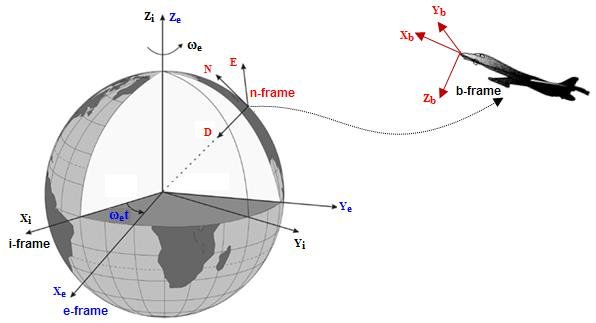
\includegraphics[width=0.65\textwidth, trim={0 0 0
    0},clip]{Reference-coordinates-frames-in-inertial-navigation-systems.png}} \caption{Physical
    System Context \cite{ins}.}
    \label{fig:ref_diag} 
\end{figure}

\textbf{Note:} This document will refer to the Navigational frame as the Earth frame, since this
follows the original documentation \cite{madgwick_ecient_nodate} and is more intuitive for the
reader.

\plt{A figure here makes sense for most SRS documents}

\subsubsection{Goal Statements}

\plt{The goal statements refine the ``Problem Description'' (Section~\ref{Sec_pd}).  A goal is a
  functional objective the system under consideration should achieve. Goals provide criteria for
  sufficient completeness of a requirements specification and for requirements pertinence. Goals
  will be refined in Section “Instanced Models” (Section~\ref{sec_instance}). Large and complex
  goals should be decomposed into smaller sub-goals.  The goals are written abstractly, with a
  minimal amount of technical language.  They should be understandable by non-domain experts.}

\noindent The goal statement is:

\begin{itemize}

\item[\textbf{GS\refstepcounter{goalnum}\thegoalnum} \label{g:calc}:] Convert sequential IMU
measurements into an orientation relative to the Earth.

\plt{One sentence description of the goal. There may be more than one. Each Goal should have a meaningful label.}

\end{itemize}

\subsection{Solution Characteristics Specification}

\plt{This section specifies the information in the solution domain of the system to be developed.
  This section is intended to express what is required in such a way that analysts and stakeholders
  get a clear picture, and the latter will accept it. The purpose of this section is to reduce the
  problem into one expressed in mathematical terms. Mathematical expertise is used to extract the
  essentials from the underlying physical description of the problem, and to collect and
  substantiate all physical data pertinent to the problem.}

\plt{This section presents the solution characteristics by successively refining models.  It starts
  with the abstract/general Theoretical Models (TMs) and refines them to the concrete/specific
  Instance Models (IMs).  If necessary there are intermediate refinements to General Definitions
  (GDs).  All of these refinements can potentially use Assumptions (A) and Data Definitions (DD).
  TMs are refined to create new models, that are called GMs or IMs. DDs are not refined; they are
  just used. GDs and IMs are derived, or refined, from other models. DDs are not derived; they are
  just given. TMs are also just given, but they are refined, not used.  If a potential DD includes a
  derivation, then that means it is refining other models, which would make it a GD or an IM.}

\plt{The above makes a distinction between ``refined'' and ``used.'' A model is refined to another
  model if it is changed by the refinement. When we change a general 3D equation to a 2D equation,
  we are making a refinement, by applying the assumption that the third dimension does not matter.
  If we use a definition, like the definition of density, we aren't refining, or changing that
  definition, we are just using it.}

\plt{The same information can be a TM in one problem and a DD in another.  It is about how the
  information is used.  In one problem the definition of acceleration can be a TM, in another it
  would be a DD.}

\plt{There is repetition between the information given in the different chunks (TM, GDs etc) with
  other information in the document.  For instance, the meaning of the symbols, the units etc are
  repeated.  This is so that the chunks can stand on their own when being read by a reviewer/user.
  It also facilitates reuse of the models in a different context.}

\noindent \plt{The relationships between the parts of the document are show in the following figure.
  In this diagram ``may ref'' has the same role as ``uses'' above.  The figure adds ``Likely
  Changes,'' which are able to reference (use) Assumptions.}

\begin{figure}[H]
  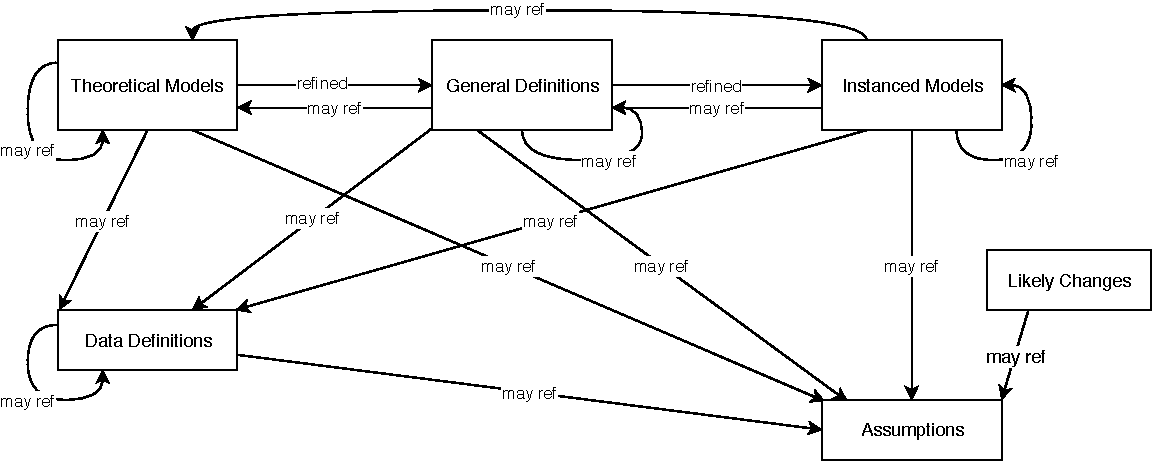
\includegraphics[scale=0.9]{RelationsBetweenTM_GD_IM_DD_A.pdf}
  \label{fig:connections}
\end{figure}

The instance models that govern \progname{} are presented in Subsection~\ref{sec_instance}.  The
information to understand the meaning of the instance models and their derivation is also presented,
so that the instance models can be verified.

\subsubsection{Types}
\begin{itemize}
    \item All scalar values in this system are $\in \mathbb{R}$.
    \item Each sensor produces a measurement vector $\in \mathbb{R}^3$.
    \item All calculations with quaternions are $\in \mathbb{R}^4$, the quaternion space. And thus
    must follow quaternion algebra \cite{quat}.
\end{itemize}

\plt{This section is optional. Defining types can make the document easier to understand.}

% \subsection{Scope Decisions}
\plt{This section is optional.}

% \subsection{Modelling Decisions}

% UPDATE LATER: Modelling of the earth magnetic field, ignoreing rotation, and variations in the
% field over distance travelled.
\plt{This section is optional.}

\subsubsection{Assumptions} \label{sec_assumpt}

\plt{The assumptions are a refinement of the scope.  The scope is general, where the assumptions are
  specific.  All assumptions should be listed, even those that domain experts know so well that they
  are rarely (if ever) written down.} \plt{The document should not take for granted that the reader
  knows which assumptions have been made. In the case of unusual assumptions, it is recommended that
  the documentation either include, or point to, an explanation and justification for the
  assumption.}
\plt{If it helps with the organization and understandability, the assumptions can be presented as sub sections.  The following sub-sections are options: background theory assumptions, helper theory assumptions, generic theory assumptions, problem specific assumptions, and rationale assumptions}

This section simplifies the original problem and helps in developing the theoretical model by
filling in the missing information for the physical system. The numbers given in the square brackets
refer to the theoretical model [TM], general definition [GD], data definition [DD], instance model
[IM], or likely change [LC], in which the respective assumption is used.

%##############################################################################
%##############################################################################
%                        ASSUMPTIONS
%##############################################################################
%##############################################################################
\begin{itemize}
    % \item[A\refstepcounter{assumpnum}\theassumpnum \label{a:relative}:] Relativistic effects can
    % be ignored. The system/IMU will is assumed to be travelling $<<$ the speed of light.
    \item[A\refstepcounter{assumpnum}\theassumpnum \label{a:gravity}:] Gravitational acceleration,
    $g_0$, is assumed to be constant in the z-axis relative to the Navigation frame.
    % \item[A\refstepcounter{assumpnum}\theassumpnum \label{a:storm}:] The operation of the system
    % will be under ``normal" weather conditions without geomagnetic interference. I.e. solar storms
    % or geomagnetic storms are not occurring during operation.
    % \item[A\refstepcounter{assumpnum}\theassumpnum \label{a:secular}:] Geomagnetic secular
    % variation is ignored. The timescale of the system's operation is assumed to be small enough
    % that variations in the magnetic field are negligible.
    \item[A\refstepcounter{assumpnum}\theassumpnum \label{a:east_mag}:] The east component of the
    magnetic field is assumed to be negligible.
    \item[A\refstepcounter{assumpnum}\theassumpnum \label{a:rotation}:] The Earth frame is
    considered inertial, and the rotation of the earth has no effect on the IMU.
    \item[A\refstepcounter{assumpnum}\theassumpnum \label{a:nonlinear}:] Sensor non-linearities are
    not considered.
    \item[A\refstepcounter{assumpnum}\theassumpnum \label{a:bandwidth}:] The sensor bandwidth is
    adequate for measuring the change in state at each time step. I.e. the frequency of the change
    in state is less than the bandwidth of the system.
    \item[A\refstepcounter{assumpnum}\theassumpnum \label{a:gsense}:] Accelerometer g-sensitivity is
    not considered. Under constant linear acceleration, the bias of an accelerometer may shift over
    time.
    \item[A\refstepcounter{assumpnum}\theassumpnum \label{a:quant}:] Quantization and analog to
    conversion error is ignored. The error from measuring of continuous phenomena with digital
    circuits will be ignored.
    \item[A\refstepcounter{assumpnum}\theassumpnum \label{a:range}:] The IMU will not experience
    phenomena outside the sensor's measurement range. I.e. the system will not accelerate beyond the
    accelerometer's measurement range.
    \item[A\refstepcounter{assumpnum}\theassumpnum \label{a:gyro}:] The gyroscope bias is assumed to
    be constant, and the sensor is calibrated and internally compensates for the bias. 
    \item[A\refstepcounter{assumpnum}\theassumpnum \label{a:mag}:] The magnetometer is assumed to
    experience no local disturbance.
    \item[A\refstepcounter{assumpnum}\theassumpnum \label{a:rigid}:] The body/IMU is assumed to be a
    rigid body.
    \item[A\refstepcounter{assumpnum}\theassumpnum \label{a:static}:] The system is assumed to be in
    a quasi-static state with little to no angular or linear acceleration.
\end{itemize}

\subsubsection{Theoretical Models}\label{sec_theoretical}

\plt{Theoretical models are sets of abstract mathematical equations or axioms for solving the
  problem described in Section ``Physical System Description'' (Section~\ref{sec_phySystDescrip}).
  Examples of theoretical models are physical laws, constitutive equations, relevant conversion
  factors, etc.}

\plt{Optionally the theory section could be divided into subsections to provide more structure and improve understandability and reusability.  Potential subsections include the following: Context theories, background theories, helper theories, generic theories, problem specific theories, final theories and rationale theories.}

This section focuses on the general equations and laws that \progname{} is based on.  \plt{Modify
the examples below for your problem, and add additional models as appropriate.}

%##############################################################################
%##############################################################################
%                       THEORETICAL MODELS
%##############################################################################
%##############################################################################

\noindent
\deftheory
% #2 refname of theory
{TM:SMM}
% #3 label
{Sensor Measurement Model}
% #4 equation
{ $\mathbf{s} = \mathbf{s}_m + \mathbf{b}_s + \bm{\mu}_s \in \mathbb{R}^n$ }
% #5 description
{ The above equation gives the model for a sensor measurement. Where $s_m$ is the true measurment,
  $b_s$ is a bias, and $\mu_s$ is an additive measurement noise.

  For this equation to apply, other forms of error such as non-linearities \aref{a:nonlinear},
bandwidth limits \aref{a:bandwidth}, quantization error \aref{a:quant}, out-of-range measurements
\aref{a:range}. }
% #6 Notes
{ The symbol for bias, $b$, should not be confused with a magnetic field measurement. }
% #7 Source
{
  \url{http://dx.doi.org/10.1109/TITS.2016.2617200}
}
% #8 Referenced by
{ \ddref{dd:acc}, \ddref{dd:gyro}, \ddref{dd:mag} }
% #9 Preconditions
{ None }
% #1 derivation - not applicable by default
{}
%##############################################################
%##############################################################
\noindent
\deftheory
% #2 refname of theory
{TM:AV}
% #3 label
{Angular Velocity}
% #4 equation
{ $\omega = \dot{\theta}$ }
% #5 description
{ The above equation gives the definition of angular velocity. Where $\omega$ is the derivitive of
the angular position, $\theta$, with repect to time. }
% #6 Notes
{ None. }
% #7 Source
{}
% #8 Referenced by
{ \dref{gd:q}, \ddref{dd:gyro} }
% #9 Preconditions
{None}
% #1 derivation - not applicable by default
{} ~\newline
%##############################################################
%##############################################################

\noindent
\deftheory
% #2 refname of theory
{TM:RK}
% #3 label
{Rotational Kinematics}
% #4 equation
{ $\theta_t = \theta_{t-1} + \omega_t \Delta t$ }
% #5 description
{ The above equation gives the definition of angular kinematics. Where $\theta_t$ is the current
angular position, $\theta_{t-1}$ is the previous position, $\Delta t$ is the period, and $\omega_t$
is the average angular velocity.

~\newline
This formular assumes that $\omega$ is constant or nearly constant during the $\Delta t$
(\aref{a:static}). }
% #6 Notes
{ None. }
% #7 Source
{}
% #8 Referenced by
{
\iref{i:o_from_gyro}
}
% #9 Preconditions
{None}
% #1 derivation - not applicable by default
{} ~\newline
%##############################################################
%##############################################################

\noindent
\deftheory
% #2 refname of theory
{TM:LA}
% #3 label
{Linear Acceleration}
% #4 equation
{ $a = \ddot{x}$ }
% #5 description
{ The above equation gives the definition of linear accerleration. Where $a$ is the second
derivitive of the linear position, $x$, with repect to time. }
% #6 Notes
{ None. }
% #7 Source
{}
% #8 Referenced by
{
    \ddref{dd:acc}
}
% #9 Preconditions
{None}
% #1 derivation - not applicable by default
{} ~\newline
%##############################################################
%##############################################################
\noindent
\deftheory
% #2 refname of theory
{TM:CF}
% #3 label
{Complimentry Filter}
% #4 equation
{ $s_f = \gamma s_1 + (1-\gamma)s_2$ }
% #5 description
{ The complimentary filter is a simple method to fuse two values with the same units together. Where
    $s_f$ is the final result of fusing the two values $s_1$ and $s_2$. The parameter $\gamma \in
    [0.0, 1.0]$, where a a value of 0 completly trusts $s_2$ and a value of 1 completly trusts
    $s_1$. }
% #6 Notes
{ None. }
% #7 Source
{}
% #8 Referenced by
{ \iref{i:o_from_comp_acc_gyro}, \iref{i:o_from_comp_all_3}. }
% #9 Preconditions
{None}
% #1 derivation - not applicable by default
{} ~\newline
%##############################################################
%##############################################################
\noindent
\deftheory
% #2 refname of theory
{TM:OFV}
% #3 label
{Orientation from vector observations.}
% #4 equation
{
\begin{align*}
\prescript{S}{F}{\mathbf{q}}_{d} &= \min\limits_{\prescript{S}{F}{\mathbf{q}}\in \mathbb{R}^4} f( \prescript{S}{F}{\mathbf{q}}, \,^F\mathbf{d}, \,^S\mathbf{s}) \\
f(\prescript{S}{F}{\mathbf{q}}, \,^F\mathbf{d}, \,^S\mathbf{s}) &= \prescript{S}{F}{\mathbf{q}} \mathbf{p}(\prescript{F}{}{\mathbf{d}}) \mathbf{p}(\prescript{S}{}{\mathbf{s}}) - \prescript{S}{}{\mathbf{s}}
\end{align*}
}
% #5 description
{ Given a measurment of a vector in a non-intertial sensor frame, $\prescript{S}{}{\mathbf{s}}$, and
a known field direction relative to a fixed-frame, $\prescript{F}{}{\mathbf{d}}$,  the quaternion
for this orientation can be approximated. However, quaternions require a complete solution
\cite{madgwick_ecient_nodate}. Thus the minimization problem presented solves for
$\prescript{S}{F}{\mathbf{q}}_\alpha$, the quaternion that represents the orientation of the sensor
frame relative to the fixed-frame. Where the subscript $d$ denotes the quatenion is minimized using
$\prescript{F}{}{\mathbf{d}}$. }
% #6 Notes
{ The function $\mathbf{p}(\mathbf{v})$ creates a pure quaternion, $(0, v_x, v_y, v_z) \in
\mathbf{R}^4$ from $\mathbf{v} \in \mathbf{R}^3$. }
% #7 Source
{\cite{madgwick_ecient_nodate}}
% #8 Referenced by
{ \iref{i:o_from_min_acc} \iref{i:o_from_min_acc_mag} }
% #9 Preconditions
{None}
% #10 derivation - not applicable by default
{}

\newpage
\subsubsection{General Definitions}\label{sec_gendef}

% This section is not applicable.

\plt{General Definitions (GDs) are a refinement of one or more TMs, and/or of other GDs.  The GDs
  are less abstract than the TMs.  Generally the reduction in abstraction is possible through
  invoking (using/referencing) Assumptions. For instance, the TM could be Newton's Law of Cooling
  stated abstracting.  The GD could take the general law and apply it to get a 1D equation.}

This section collects the laws and equations that will be used in building the instance models.

\plt{Some projects may not have any content for this section, but the section heading should be
  kept.}  \plt{Modify the examples below for your problem, and add additional definitions as
  appropriate.}

~\newline
%##############################################################################
%##############################################################################
%                       GENERAL MODELS
%##############################################################################
%##############################################################################
\noindent
\begin{minipage}{\textwidth}
\renewcommand*{\arraystretch}{1.5}
\begin{tabular}{| p{\colAwidth} | p{\colBwidth}|}
\hline
\rowcolor[gray]{0.9}
Number& GD\refstepcounter{defnum}\thedefnum \label{gd:q}\\
\hline
Label &\bf Angular velocity as a Quaternion. \\
\hline
SI Units&\si{\radian\per\second}\\
\hline
Equation&  $\dot{\mathbf{q}} = \frac{1}{2} \mathbf{q} \mathbf{p}(\bm{\omega})$ \\
\hline
Description & The above equation gives the model for the evolution of the orientation over time.
Where $\mathbf{q}$ is a unit quaternion, $\dot{\mathbf{q}}$ is the rate of change of the quaternion,
and $\mathbf{p}(\bm{\omega})$ is the unitary pure quaternion associated to the angular velocity
$\mathbf{p}(\bm{\omega}) = (0, \omega_x,  \omega_y,  \omega_z)$.

~\newline
For this equation to apply, the object/IMU must be a rigid body (\aref{a:rigid}).

~\newline
\textbf{Note:} Quaternion multiplication uses the Hamilton product \cite{hamilton}. \\
\hline
  Source & \cite{mahoney} \\
  \hline
  Ref.\ By & \iref{i:o_from_gyro}.\\
  \hline
\end{tabular}
\end{minipage}\\

\subsubsection{Data Definitions}\label{sec_datadef}

\plt{The Data Definitions are definitions of symbols and equations that are given for the problem.
  They are not derived; they are simply used by other models.  For instance, if a problem depends on
  density, there may be a data definition for the equation defining density.  The DDs are given
  information that you can use in your other modules.}

\plt{All Data Definitions should be used (referenced) by at least one other model.}

This section collects and defines all the data needed to build the instance models. The dimension of
each quantity is also given.  \plt{Modify the examples below for your problem, and add additional
definitions as appropriate.}

~\newline
%##############################################################################
%##############################################################################
%                       Data Definitions
%##############################################################################
%##############################################################################
\noindent
\begin{minipage}{\textwidth}
\renewcommand*{\arraystretch}{1.5}
\begin{tabular}{| p{\colAwidth} | p{\colBwidth}|}
\hline
\rowcolor[gray]{0.9}
Number& DD\refstepcounter{datadefnum}\thedatadefnum \label{dd:acc}\\
\hline
Label& \bf Acceleration Measurement\\
\hline
Symbol &$a$\\
\hline
  SI Units & \si{\meter\per\square\second}\\
  \hline 

  Equation& $\mathbf{a} = \mathbf{a}_m + \mathbf{b}_a + \bm{\mu}_a \in \mathbb{R}^3 $\\
  \hline
  Description & $\mathbf{a_m}$ is the true acceleration vector defined by \tref{TM:LA}.
  $\mathbf{b_a}$ is the bias for each axis of the accelerometer. $\mu_a$ is the additive noise
  vector. The accelerometer measurement vector $\mathbf{a}$ is the sum of the components above. 
  
  % This assumes that body/IMU does not deflect during acceleration \aref{a:rigid}.
  
  ~\newline
  Often, acceleration measurements will have the reference frame and time step added. Example:
  $\prescript{S}{}{\mathbf{a}}_t$. \\
  \hline
  Sources&  \\
  \hline
  Ref.\ By & \iref{i:o_from_min_acc}, \iref{i:o_from_min_acc_mag}, \iref{i:o_from_comp_acc_gyro}. \\
  \hline
\end{tabular}
\end{minipage}\\

~\newline
\noindent
\begin{minipage}{\textwidth}
\renewcommand*{\arraystretch}{1.5}
\begin{tabular}{| p{\colAwidth} | p{\colBwidth}|}
\hline
\rowcolor[gray]{0.9}
Number& DD\refstepcounter{datadefnum}\thedatadefnum \label{dd:gyro}\\
\hline
Label& \bf Gyroscope Measurement\\
\hline
Symbol &$\bm{\omega}$\\
\hline
  SI Units & \si{\radian\per\second}\\
  \hline 

  Equation& $\bm{\omega} = \bm{\omega}_m + \mathbf{b}_g+ \bm{\mu}_g \in \mathbb{R}^3 $\\
  \hline
  Description & $\bm{\omega}_m$ is the true gyroscopic rate vector defined by \tref{TM:AV}.
  $\mathbf{b}_g$ is the bias for each axis of the gyroscope. $\mu_g$ is the additive noise vector.
  The gyroscope measurement vector $\bm{\omega}$ is the sum of the components above.
    
  ~\newline
  Often, gyroscope measurements will have the reference frame and time step added. Example:
  $\prescript{S}{}{\bm{\omega}}_t$. \\
  \hline
  Sources&  \\
  \hline
  Ref.\ By & \iref{i:o_from_gyro}, \iref{i:o_from_comp_acc_gyro}, \iref{i:o_from_comp_all_3}. \\
  \hline
\end{tabular}

~\newline
\end{minipage}\\
~\newline
\noindent
\begin{minipage}{\textwidth}
\renewcommand*{\arraystretch}{1.5}
\begin{tabular}{| p{\colAwidth} | p{\colBwidth}|}
\hline
\rowcolor[gray]{0.9}
Number& DD\refstepcounter{datadefnum}\thedatadefnum \label{dd:mag}\\
\hline
Label& \bf Magnetometer Measurement\\
\hline
Symbol &$\mathbf{m}$\\
\hline
  SI Units & \si{\tesla}\\
  \hline 

  Equation& $\mathbf{m} = \mathbf{m}_m + \mathbf{b}_m + \bm{\mu}_m \in \mathbb{R}^3 $\\
  \hline
  Description & $\mathbf{m}_m$ is the true magnetometer vector. $\mathbf{b}_m$ is the bias for each
  axis of the magnetometer. $\mu_m$ is the additive noise vector. The magnetometer measurement
  vector $\mathbf{m}$ is the sum of the components above.
    
  ~\newline
  Often, magnetometer measurements will have the reference frame and time step added. Example:
  $\prescript{S}{}{\mathbf{m}}_t$. \\
  \hline
  Sources&  \\
  \hline
  Ref.\ By & \iref{i:o_from_min_acc_mag}, \iref{i:o_from_comp_all_3}. \\
  \hline
\end{tabular}
\end{minipage}\\

\subsubsection{Data Types}\label{sec_datatypes}

This section is not applicable.

\plt{This section is optional.  In many scientific computing programs it isn't necessary, since the
  inputs and outpus are straightforward types, like reals, integers, and sequences of reals and
  integers.  However, for some problems it is very helpful to capture the type information.}

\plt{The data types are not derived; they are simply stated and used by other models.}

\plt{All data types must be used by at least one of the models.}

\plt{For the mathematical notation for expressing types, the recommendation is to use the notation
  of~\cite{HoffmanAndStrooper1995}.}

% This section collects and defines all the data types needed to document the models.
\plt{Modify the examples below for your problem, and add additional definitions as appropriate.}

% ~\newline

% \noindent \begin{minipage}{\textwidth} \renewcommand*{\arraystretch}{1.5} \begin{tabular}{|
% p{\colAwidth} | p{\colBwidth}|} \hline \rowcolor[gray]{0.9} Type Name & Name for Type\\
%   \hline Type Def & mathematical definition of the type\\
%   \hline Description & description here
%   \\
%   \hline Sources & Citation here, if the type is borrowed from another source\\
%   \hline \end{tabular} \end{minipage}\\

\subsubsection{Instance Models} \label{sec_instance}    

\plt{The motivation for this section is to reduce the problem defined in ``Physical System
  Description'' (Section~\ref{sec_phySystDescrip}) to one expressed in mathematical terms. The IMs
  are built by refining the TMs and/or GDs.  This section should remain abstract.  The SRS should
  specify the requirements without considering the implementation.}

This section transforms the problem defined in Section~\ref{Sec_pd} into one which is expressed in
mathematical terms. It uses concrete symbols defined in Section~\ref{sec_datadef} to replace the
abstract symbols in the models identified in Sections~\ref{sec_theoretical} and~\ref{sec_gendef}.

The goal \gsref{g:calc} is solved by combining the results from \iref{i:o_from_comp_all_3} when all
three sensor measurements are provided, and \iref{i:o_from_comp_acc_gyro} when the magnetometer is
omitted. \plt{reference your instance models}

~\newline
%##############################################################################
%##############################################################################
%                       INSTANCE MODELS
%##############################################################################
%##############################################################################
%Instance Model 1
\begin{minipage}{\textwidth}
\renewcommand*{\arraystretch}{1.5}
\begin{tabular}{| p{\colAwidth} | p{\colBwidth}|}
  \hline
  \rowcolor[gray]{0.9}
  Number& IM\refstepcounter{instnum}\theinstnum \label{i:o_from_gyro}\\
  \hline
  Label& \bf Orientation from Gyro measurements\\
  \hline
  Input& $\mathbf{q}_{t-1}, \prescript{S}{}{\bm{\omega}_t}, \Delta t$ \\
  & The input is constrained so that $|\mathbf{\omega}_t| \leq \mathbf{\omega}_{\text{max}}$
  (\aref{a:range})\\
  \hline
  Output &  $\mathbf{q}_{\omega,t} = \mathbf{q}_{t-1} + \dot{\mathbf{q}_t} \Delta t$ \\
        & $ \phantom{\mathbf{q}_t} = \mathbf{q}_{t-1} +
        \frac{1}{2}\mathbf{q}_{t-1}\mathbf{p}(\prescript{S}{}{\bm{\omega}_t}) \Delta t$\\
  \hline
  Description& The current orientation $\mathbf{q}_{\omega,t}$ is computed using \tref{TM:RK}. Where
  $\mathbf{q}_{t-1}$ the previous orientation and $\dot{\mathbf{q}_t}$ from \dref{gd:q}, which
  requires $\prescript{S}{}{\bm{\omega}_t}$, the current gyroscope measurement in the sensor frame.
  Where $\Delta t$ is the period since the last calculation.

  ~\newline
  The additional subscript $\omega$ denotes that the quaternion is computed from angular rate, \\
  \hline
  Sources & \cite{madgwick_ahrs}, \cite{madgwick_ecient_nodate} \\
  \hline
  Ref.\ By & \iref{i:o_from_comp_acc_gyro}, \iref{i:o_from_comp_all_3}.\\
  \hline
\end{tabular}
\end{minipage}\\

~\newline
%Instance Model 2
\begin{minipage}{\textwidth}
\renewcommand*{\arraystretch}{1.5}
\begin{tabular}{| p{\colAwidth} | p{\colBwidth}|}
  \hline
  \rowcolor[gray]{0.9}
  Number& IM\refstepcounter{instnum}\theinstnum \label{i:o_from_min_acc}\\
  \hline
  Label& \bf Orientation from Accelerometer measurements\\
  \hline
  Input & $\prescript{S}{E}{\mathbf{q}},  \prescript{E}{}{\mathbf{g}}_0,
  \prescript{S}{}{\mathbf{a}}$ \\
  & The gravity vector is normalized to $\mathbf{g} = (0, 0, 1)^T$ (\aref{a:gravity}). The
  acceleration measurement is in the sensor frame, and constrained to $|a| \leq a_\text{max}$
  (\aref{a:range}).\\
  \hline
  Output  &  $\prescript{S}{E}{\mathbf{q}}_g = \min\limits_{\prescript{S}{E}{\mathbf{q}}\in
  \mathbb{R}^4} f( \prescript{S}{E}{\mathbf{q}}, \prescript{E}{}{\mathbf{g}}_0, \,^S\mathbf{a}) $\\
 % & $f( \prescript{S}{E}{\mathbf{q}}, \prescript{E}{}{\mathbf{g}}_0, \,^S\mathbf{a}) =
 % \prescript{S}{F}{\mathbf{q}} \mathbf{p}(\prescript{E}{}{\mathbf{g}}_0)
 % \mathbf{p}(\prescript{S}{}{\mathbf{a}}) - \prescript{S}{}{\mathbf{a}}$ \\
  \hline
  Description & Using the known gravitational field in the Earth frame, and a measured sensor-frame
  acceleration under \aref{a:static}, the orientation, $\prescript{S}{E}{\mathbf{q}}_g$, can be
  computed using \tref{TM:OFV}.
    
  ~\newline
  Since the gravity vector only has one component, this method cannot accurately estimate the
  heading angle, only pitch and role are accurate.

  ~\newline
  The Earth frame is is assumed to be inertial \aref{a:rotation}. \\
  \hline
  Sources & \cite{madgwick_ahrs}, \cite{madgwick_ecient_nodate} \\
  \hline
  Ref.\ By & \iref{i:o_from_comp_acc_gyro}.\\
  \hline
\end{tabular}
\end{minipage}\\

%Instance Model 3
~\newline
\begin{minipage}{\textwidth}
\renewcommand*{\arraystretch}{1.5}
\begin{tabular}{| p{\colAwidth} | p{\colBwidth}|}
  \hline
  \rowcolor[gray]{0.9}
  Number& IM\refstepcounter{instnum}\theinstnum \label{i:o_from_min_acc_mag}\\
  \hline
  Label& \bf Orientation from Accelerometer and Magnetometer\\
  \hline
  Input& $\prescript{S}{E}{\mathbf{q}}, \prescript{E}{}{\mathbf{g}}_0, \prescript{S}{}{\mathbf{a}},
  \,^E\mathbf{b}, \,^S\mathbf{m}$\\
    & The gravity vector is normalized to $\prescript{E}{}{\mathbf{g}}_0 = (0, 0, 1)^T$
    (\aref{a:gravity}). Following \aref{a:east_mag} the magnetic field vector is simplified to
    $\mathbf{b} = (b_x, 0, b_z)^T$. The acceleration  and magnetometer measurements are in the
    sensor frame.\\
  \hline
  Output  &  $\prescript{S}{E}{\mathbf{q}}_{g, b} = \min\limits_{\prescript{S}{E}{\mathbf{q}}\in
  \mathbb{R}^4} f_{g,b}( \prescript{S}{E}{\mathbf{q}},  \prescript{E}{}{\mathbf{g}}_0,
  \,^S\mathbf{a}, \,^E\mathbf{b}, \,^S\mathbf{m}) $\\

& $ f_{g,b}( \prescript{S}{E}{\mathbf{q}},  \prescript{E}{}{\mathbf{g}}_0, \,^S\mathbf{a},
\,^E\mathbf{b}, \,^S\mathbf{m})= \begin{bmatrix}f_g( \prescript{S}{E}{\mathbf{q}},
\prescript{E}{}{\mathbf{g}}_0, \,^S\mathbf{a}) \\ f_b( \prescript{S}{E}{\mathbf{q}}, \,^E\mathbf{b},
\,^S\mathbf{m})\end{bmatrix}$ \\
  
  \hline
  Description & Combining \iref{i:o_from_min_acc} with the known magnetic field in the Earth frame
  and a measured sensor-frame magnetic field, the orientation, $\prescript{S}{E}{\mathbf{q}}_{g,
  b}$, can be computed using \tref{TM:OFV}. \\
  \hline
  Sources & \cite{madgwick_ahrs}, \cite{madgwick_ecient_nodate} \\
  \hline
  Ref.\ By & \iref{i:o_from_comp_all_3}. \\
  \hline
\end{tabular}
\end{minipage}\\

~\newline
%Instance Model 4
\begin{minipage}{\textwidth}
\renewcommand*{\arraystretch}{1.5}
\begin{tabular}{| p{\colAwidth} | p{\colBwidth}|}
    \hline
    \rowcolor[gray]{0.9}
    Number& IM\refstepcounter{instnum}\theinstnum \label{i:o_from_comp_acc_gyro}\\
    \hline
    Label& \bf Orientation from Accelerometer and Gyroscope\\
    \hline
    Input& $\prescript{S}{E}{\mathbf{q}}_{\omega, t}, \prescript{S}{E}{\mathbf{q}}_{g, t},
    \prescript{S}{}{\mathbf{a}}_t, \prescript{E}{}{\mathbf{g}}_0, \prescript{S}{}{\bm{\omega}_t},
    \Delta t$\\
    & The sensor measurements are from the current time step, and the quaternion estimate is from
    the previous time step. \\
    \hline
    Output & $\prescript{S}{E}{\mathbf{q}}_{t} = \gamma \prescript{S}{E}{\mathbf{q}}_{\omega, t} +
    (1-\gamma) \prescript{S}{E}{\mathbf{q}}_{g, t}$\\
    \hline
    Description& Combining estimates from \iref{i:o_from_gyro} and \iref{i:o_from_min_acc} using the
    complementary filter from \tref{TM:CF} produces a quaternion output using accelerometer and
    gyroscope measurements. \\
    \hline
    Sources & \cite{madgwick_ecient_nodate}\\
    \hline
    Ref.\ By & \rref{r:calculate2}.\\
    \hline
\end{tabular}
\end{minipage}\\

~\newline
%Instance Model 5
\begin{minipage}{\textwidth}
\renewcommand*{\arraystretch}{1.5}
\begin{tabular}{| p{\colAwidth} | p{\colBwidth}|}
\hline
\rowcolor[gray]{0.9}
Number& IM\refstepcounter{instnum}\theinstnum \label{i:o_from_comp_all_3}\\
\hline
Label& \bf Orientation from Accelerometer, Gyroscope, and Magnetometer\\
\hline
Input& $\prescript{S}{E}{\mathbf{q}}_{\omega, t}, \prescript{S}{E}{\mathbf{q}}_{(g,b), t},
\prescript{S}{}{\mathbf{a}}_t, \prescript{E}{}{\mathbf{g}}_0, \prescript{S}{}{\bm{\omega}_t}, \Delta
t$\\
& The sensor measurements are from the current time step, and the quaternion estimate is from the
previous time step. \\
\hline
Output & $\prescript{S}{E}{\mathbf{q}}_{t} = \gamma \prescript{S}{E}{\mathbf{q}}_{\omega, t} +
(1-\gamma) \prescript{S}{E}{\mathbf{q}}_{(g,b), t}$\\
\hline
Description& Combining estimates from \iref{i:o_from_gyro} and \ref{i:o_from_min_acc_mag} using the
complementary filter from \tref{TM:CF} produces a quaternion output using accelerometer and
gyroscope measurements. \\
\hline
Sources & \cite{madgwick_ecient_nodate} \\
\hline
Ref.\ By & \rref{r:calculate1}.\\
\hline
\end{tabular}
\end{minipage}\\

% \subsubsection*{Derivation of ...}

\plt{The derivation shows how the IM is derived from the TMs/GDs.  In cases where the derivation
  cannot be described under the Description field, it will be necessary to include this subsection.}

\subsubsection{Input Data Constraints} \label{sec_DataConstraints}    

Table~\ref{TblInputVar} shows the data constraints on the input output variables.  The column for
physical constraints gives the physical limitations on the range of values that can be taken by the
variable.  The column for software constraints restricts the range of inputs to reasonable values.
The software constraints will be helpful in the design stage for picking suitable algorithms.  The
constraints are conservative, to give the user of the model the flexibility to experiment with
unusual situations.  The column of typical values is intended to provide a feel for a common
scenario.  The uncertainty column provides an estimate of the confidence with which the physical
quantities can be measured.  This information would be part of the input if one were performing an
uncertainty quantification exercise.

The specification parameters in Table~\ref{TblInputVar} are listed in Table~\ref{TblSpecParams}.

\begin{table}[!h]
  \caption{Input Variables} \label{TblInputVar}
  \renewcommand{\arraystretch}{1.2}
\noindent \begin{longtable*}{l l l l c} 
\toprule
\textbf{Var} & \textbf{Physical Constraints} & \textbf{Software Constraints} & \textbf{Typical
Value} & \textbf{Uncertainty}\\
\midrule 
    $\Delta t$ & $\Delta t > 0$ & $\Delta t_{\text{min}} \leq \Delta t \leq \Delta t_{\text{max}}$ &
    10 \si[per-mode=symbol] {\milli\second} & - \\
    $a$ & $-\infty < a < \infty$ & $|a| \leq a_{\text{max}}$ & 9.81 \si[per-mode=symbol]
    {\meter\per\square\second} & See sensor datasheet. \\
    $m$ & $-\infty < m < \infty$ & $|m| \leq m_{\text{max}}$ & 25 \si[per-mode=symbol] {\micro
    \tesla} & See sensor datasheet. \\
    $\omega$ & $-\infty < \omega < \infty$ & $|\mathbf{\omega}| \leq \omega_{\text{max}}$ & 1.0
    \si[per-mode=symbol] {\radian\per\second} & See sensor datasheet. \\
    $\gamma$ & - & $0.0 \leq \gamma \leq 1.0$ & 0.5 & - \\
\bottomrule
\end{longtable*}
\end{table}

% \noindent \begin{description} \item[(*)] \plt{you might need to add some notes or clarifications}
% \end{description}

\begin{table}[!h]
\caption{Specification Parameter Values} \label{TblSpecParams}
\renewcommand{\arraystretch}{1.2}
\noindent \begin{longtable*}{l l} 
\toprule
\textbf{Var} & \textbf{Value} \\
\midrule 
    $\Delta t_\text{min}$ & 1 \si{\milli\second}\\
    $\Delta t_\text{max}$ & 100000 \si{\milli\second}\\
    $a_\text{max}$ & See sensor datasheet [\si{\meter\per\square\second}].\\
    $m_\text{max}$ & See sensor datasheet [\si{\tesla}].\\
    $\omega_\text{max}$ & See sensor datasheet [\si{\radian\per\second}].\\
\bottomrule
\end{longtable*}
\end{table}

\subsubsection{Properties of a Correct Solution} \label{sec_CorrectSolution}

\noindent
A correct solution must be a valid orientation representation, calculation results are unit
quaternions and can be optionally converted to another attitude representation.

\plt{These properties are in addition to the stated requirements.  There is no need to repeat the
requirements here.  These additional properties may not exist for every problem.  Examples include
conservation laws (like conservation of energy or mass) and known constraints on outputs, which are
usually summarized in tabular form.  A sample table is shown in Table~\ref{TblOutputVar}}

\begin{table}[!h]
\caption{Output Variables} \label{TblOutputVar}
\renewcommand{\arraystretch}{1.2}
\noindent \begin{longtable*}{l l} 
  \toprule
  \textbf{Var} & \textbf{Physical Constraints} \\
  \midrule 
  $\mathbf{q}_t$ & $| \mathbf{q}_t | = 1$ \\
  \bottomrule
\end{longtable*}
\end{table}

\plt{This section is not for test cases or techniques for verification and validation.  Those topics
  will be addressed in the Verification and Validation plan.}

\section{Requirements} \label{sec:reqs}

\plt{The requirements refine the goal statement.  They will make heavy use of references to the
  instance models.}

This section provides the functional requirements, the business tasks that the software is expected
to complete, and the nonfunctional requirements, the qualities that the software is expected to
exhibit.

\subsection{Functional Requirements}

\begin{itemize}
    \item[R\refstepcounter{reqnum}\thereqnum \label{r:inputs}:] \plt{Requirements for the inputs
    that are supplied by the user.  This information has to be explicit.} The user shall provide
    system inputs at initialization and every time step as listed below.
    
    \textbf{Initialization}: the sensor sampling time $\Delta t$, the local magnetic field intensity
    vector, the gain parameter $\gamma$, the desired output format, and the initial orientation if
    magnetometer measurements are not present.

    \textbf{Each time step}: temporally synchronized (accelerometer, magnetometer, gyroscope)
    measurements or (accelerometer, gyroscope) measurements.
    
    \item[R\refstepcounter{reqnum}\thereqnum \label{r:calculate1}:] \progname{} shall calculate the
    orientation relative to the Earth frame when provided with  accelerometer, gyroscope, and
    magnetometer measurements.
    
    \item[R\refstepcounter{reqnum}\thereqnum \label{r:calculate2}:] \progname{} shall calculate the
    yaw and pitch components of the orientation relative to the Earth frame when provided with
    accelerometer and gyroscope measurements.
    
    \item[R\refstepcounter{reqnum}\thereqnum \label{r:output}:] \plt{Output related requirements.}
    \progname{} shall output the orientation in the user specified format.
\end{itemize}

\plt{Every IM should map to at least one requirement, but not every requirement has to map to a corresponding IM.}

\subsection{Nonfunctional Requirements}

\plt{List your nonfunctional requirements.  You may consider using a fit criterion to make them
  verifiable.} \plt{The goal is for the nonfunctional requirements to be unambiguous, abstract and
  verifiable.  This isn't easy to show succinctly, so a good strategy may be to give a ``high
  level'' view of the requirement, but allow for the details to be covered in the Verification and
  Validation document.} \plt{An absolute requirement on a quality of the system is rarely needed.
  For instance, an accuracy of 0.0101 \% is likely fine, even if the requirement is for 0.01 \%
  accuracy.  Therefore, the emphasis will often be more on describing now well the quality is
  achieved, through experimentation, and possibly theory, rather than meeting some bar that was
  defined a priori.} \plt{You do not need an entry for correctness in your NFRs.  The purpose of the
  SRS is to record the requirements that need to be satisfied for correctness. Any statement of
  correctness would just be redundant. Rather than discuss correctness, you can characterize how far
  away from the correct (true) solution you are allowed to be.  This is discussed under accuracy.}

\begin{itemize}
    \item[NFR\refstepcounter{nfrnum}\thenfrnum \label{nfr:accuracy}:] \textbf{Accuracy}
        \plt{Characterize the accuracy by giving the context/use for the software.  Maybe something
        like, ``The accuracy of the computed solutions should meet the level needed for
        $<$engineering or scientific application$>$.  The level of accuracy achieved by \progname{}
        shall be described following the procedure given in Section~X of the Verification and
        Validation Plan.''  A link to the VnV plan would be a nice extra.} The level of accuracy
        achieved by \progname{} shall be described in the Verification and Validation plan (not yet
        created).
    
    \item[NFR\refstepcounter{nfrnum}\thenfrnum \label{nfr:usability}:] \textbf{Usability}:
      \progname{} shall follow standard coding conventions such that the Application programming
      Interface (API) is clearly understood by a typical user. \plt{Characterize the usability by
      giving the context/use for the software. You should likely reference the user characteristics
      section.  The level of usability achieved by the software shall be described following the
      procedure given in Section~X of the Verification and Validation Plan.  A link to the VnV plan
      would be a nice extra.}
    
    \item[NFR\refstepcounter{nfrnum}\thenfrnum \label{nfr:maintainability}:]
    \textbf{Maintainability}: The effort required to make any of the likely changes listed for
    \progname{} should be less than $\eta$ of the original development time.
    
    \item[NFR\refstepcounter{nfrnum}\thenfrnum \label{nfr:portability}:]
      \textbf{Portability}: \progname{} shall compile (if necessary) and run on Ubuntu 20.04, macOS
      14 Sonoma, and Win 10/11.
  
\plt{This NFR is easier to write than the others.  The systems that \progname{} should run on should
    be listed here.  When possible the specific versions of the potential operating environments
    should be given.  To make the NFR verifiable a statement could be made that the tests from a
    given section of the VnV plan can be successfully run on all of the possible operating
    environments.}
% \item Other NFRs that might be discussed include verifiability, understandability and reusability.
\end{itemize}

\subsection{Rationale}

The scope and assumptions in this document reflect realistic assumptions for a real-world sensors
and systems. For small drones and robotics applications, the accuracy and quality of the sensors are
too low to require accounting for the rotation of the Earth.

Typical values reflect values in recreational and hobby drones and robots.

\plt{Provide a rationale for the decisions made in the documentation.  Rationale should be provided
for scope decisions, modelling decisions, assumptions and typical values.}

\section{Likely Changes} \label{sec:likely_changes}

\begin{itemize}
    % \item[LC\refstepcounter{lcnum}\thelcnum\label{lc:list}:] Add functionality to process a list
    % of sequential measurements and output a list of orientations instead of one at a time.
    \item[LC\refstepcounter{lcnum}\thelcnum\label{lc:gyro}:] Add online gyroscope bias compensation.
    This removes \aref{a:gyro}.
    \item[LC\refstepcounter{lcnum}\thelcnum\label{lc:mag}:] Add magnetic disturbance compensation.
    This removes \aref{a:mag}.
\end{itemize}

\section{Unlikely Changes} \label{sec:unlikely_changes}

None.

% \noindent \begin{itemize} \item[LC\refstepcounter{lcnum}\thelcnum\label{UC_meaningfulLabel}:]
% \plt{Give the unlikely changes.  The design can assume that the changes listed will not occur.}
% \end{itemize}

\section{Traceability Matrices and Graphs} \label{sec:trace}

The purpose of the traceability matrices is to provide easy references on what has to be
additionally modified if a certain component is changed.  Every time a component is changed, the
items in the column of that component that are marked with an ``X'' may have to be modified as well.
Table~\ref{Table:A_trace} shows the dependencies of theoretical models, general definitions, data
definitions, instance models, and likely changes on the assumptions.  Table~\ref{Table:trace} shows
the dependencies of theoretical models, general definitions, data definitions, and instance models
with each other. Table~\ref{Table:R_trace} shows the dependencies of instance models, requirements,
and data constraints on each other.

\plt{You will have to modify these tables for your problem.}
\plt{The traceability matrix is not generally symmetric.  If GD1 uses A1, that means that GD1's
  derivation or presentation requires invocation of A1.  A1 does not use GD1.  A1 is ``used by''
  GD1.} \plt{The traceability matrix is challenging to maintain manually.  Please do your best.  In
  the future tools (like Drasil) will make this much easier.}

% \begin{landscape}
\begin{table}[h!]
\centering
\begin{tabular}{|c|c|c|c|c|c|c|c|c|c|c|c|c|}
\hline
	& \aref{a:gravity}
	&\aref{a:east_mag}&\aref{a:rotation}&\aref{a:nonlinear}&\aref{a:bandwidth}&\aref{a:gsense}&\aref{a:quant}&\aref{a:range}&\aref{a:gyro}&\aref{a:mag}
	&\aref{a:rigid}& \aref{a:static} \\
\hline
\tref{TM:SMM}               & & & & X& X& & X& X& & & & \\ \hline
\tref{TM:AV}                & & & & & & & & & & & X& \\ \hline
\tref{TM:RK}                & & & & & & & & & & & X&X \\ \hline
\tref{TM:LA}                & & & & & & & & & & & & \\ \hline
\tref{TM:CF}                & & & & & & & & & & & & \\ \hline
\tref{TM:OFV}               & & & & & & & & & & & & \\ \hline
\dref{gd:q}                 & & & & & & & & & & & X& \\ \hline
\ddref{dd:acc}              & & & & X& X& X& X& X& & & & \\ \hline
\ddref{dd:gyro}             & & & X& X& X& & X& X& X& & & \\ \hline
\ddref{dd:mag}              & & & & X& X& & X& X& & X& & \\ \hline
\iref{i:o_from_gyro}        & & & X& X& X& & X& X& X& & X&X \\ \hline
\iref{i:o_from_min_acc}     & X& & & X& X& X& X& X& & & &X \\ \hline
\iref{i:o_from_min_acc_mag} & X& X& & X& X& X& X& X& & X& &X \\ \hline
\iref{i:o_from_comp_acc_gyro}&X& & X& X& X& X& X& X& X& & X&X \\ \hline
\iref{i:o_from_comp_all_3}  & X& X& X& X& X& X& X& X& X& X& X&X  \\ \hline
\lcref{lc:gyro}             & & & & & & & & & X& & & \\ \hline
\lcref{lc:mag}              & & & & & & & & & & X& & \\ \hline
\end{tabular}
\caption{Traceability Matrix Showing the Connections Between Assumptions and Other Items}
\label{Table:A_trace}
\end{table}
% \end{landscape}

% \afterpage{
\begin{landscape}
\begin{table}[h!]
\centering
\begin{tabular}{|c|c|c|c|c|c|c|c|c|c|c|c|c|c|c|c|}
\hline        
    & \tref{TM:SMM} &\tref{TM:AV}  &\tref{TM:RK}  &\tref{TM:LA}  &\tref{TM:CF}  &\tref{TM:OFV}
    &\dref{gd:q}   &\ddref{dd:acc}&\ddref{dd:gyro}&\ddref{dd:mag}&\iref{i:o_from_gyro}
    &\iref{i:o_from_min_acc}      &\iref{i:o_from_min_acc_mag}  &\iref{i:o_from_comp_acc_gyro}
    &\iref{i:o_from_comp_all_3} \\ \hline
    \tref{TM:SMM}                 & & & & & & & & & & & & & & &  \\ \hline
    \tref{TM:AV}                  & & & & & & & & & & & & & & &  \\ \hline
    \tref{TM:RK}                  & &X& & & & & & & & & & & & &  \\ \hline
    \tref{TM:LA}                  & & & & & & & & & & & & & & &  \\ \hline
    \tref{TM:CF}                  & & & & & & & & & & & & & & &  \\ \hline
    \tref{TM:OFV}                 & & & & & & & & & & & & & & &  \\ \hline
    \dref{gd:q}                   & &X& & & & & & & & & & & & &  \\ \hline
    \ddref{dd:acc}                &X& & &X& & & & & & & & & & &  \\ \hline
    \ddref{dd:gyro}               &X&X& & & & & & & & & & & & &  \\ \hline
    \ddref{dd:mag}                &X& & & & & & & & & & & & & &  \\ \hline
    \iref{i:o_from_gyro}          &X&X&X& & & &X& & & & & & & &  \\ \hline
    \iref{i:o_from_min_acc}       &X& & &X& &X& &X& & & & & & &  \\ \hline
    \iref{i:o_from_min_acc_mag}   &X& & &X& &X& & & &X& & & & &  \\ \hline
    \iref{i:o_from_comp_acc_gyro} &X&X&X&X&X&X&X&X&X& &X&X& & &  \\ \hline
    \iref{i:o_from_comp_all_3}    &X&X&X&X&X&X&X&X&X&X&X& &X& &  \\ \hline
\end{tabular}
\caption{Traceability Matrix Showing the Connections Between Items of Different Sections}
\label{Table:trace}
\end{table}
\end{landscape}
% }

\begin{table}[h!]
\centering
\begin{tabular}{|c|c|c|c|c|c|c|c|c|c|}
\hline
	&\iref{i:o_from_gyro}         &\iref{i:o_from_min_acc}      &\iref{i:o_from_min_acc_mag}
	&\iref{i:o_from_comp_acc_gyro} &\iref{i:o_from_comp_all_3} & \rref{r:inputs}   &
	\rref{r:calculate1}  & \rref{r:calculate2}& \rref{r:output}    \\
\hline
\iref{i:o_from_gyro}         & & & & & & & & & \\ \hline
\iref{i:o_from_min_acc}      & & & & & & & & & \\ \hline
\iref{i:o_from_min_acc_mag}  & & & & & & & & & \\ \hline
\iref{i:o_from_comp_acc_gyro}& & & & & &X& &X& \\ \hline
\iref{i:o_from_comp_all_3}   & & & & & &X&X& & \\ \hline
\rref{r:inputs}              & & & & & & & & & \\ \hline
\rref{r:calculate1}          & & & & & & & & & \\ \hline
\rref{r:calculate2}          & & & & & & & & & \\ \hline
\rref{r:output}              & & & & & & & & & \\ \hline
\end{tabular}
\caption{Traceability Matrix Showing the Connections Between Requirements and Instance Models}
\label{Table:R_trace}
\end{table}

% The purpose of the traceability graphs is also to provide easy references on what has to be
% additionally modified if a certain component is changed.  The arrows in the graphs represent
% dependencies. The component at the tail of an arrow is depended on by the component at the head of
% that arrow. Therefore, if a component is changed, the components that it points to should also be
% changed. Figure~\ref{Fig_ATrace} shows the dependencies of theoretical models, general
% definitions, data definitions, instance models, likely changes, and assumptions on each other.
% Figure~\ref{Fig_RTrace} shows the dependencies of instance models, requirements, and data
% constraints on each other.

\section{Development Plan} \label{sec:dev_plan}

N/A.

\plt{This section is optional.  It is used to explain the plan for developing the software.  In
particular, this section gives a list of the order in which the requirements will be implemented. In
the context of a course  this is where you can indicate which requirements will be implemented as
part of the course, and which will be ``faked'' as future work.  This section can be organized as a
prioritized list of requirements, or it could should the requirements that will be implemented for
``phase 1'', ``phase 2'', etc.}

\section{Values of Auxiliary Constants}

\begin{table}[!h]
\caption{Table of Constants} \label{t:aux_const}
\renewcommand{\arraystretch}{1.2}
\noindent \begin{longtable*}{l l} 
\toprule
\textbf{Var} & \textbf{Value} \\
\midrule 
    $\eta$ & $\cfrac{1}{21}$ \vspace{2mm} \\ 
    $\mathbf{g}_0$ & $(0, 0, 9.81)^T$ \\
    ${}^E\mathbf{b}$ & $(16676.8, -3050.9, 49916.9)^T$\\
\bottomrule
\end{longtable*}
\end{table}

\textbf{Note:} Magnetic field values were calculated from the World Magnetic Model (WMM) \cite{wmm}
for Toronto, ON. Other locations may have different values.

\plt{Show the values of the symbolic parameters introduced in the report.}

\newpage

\bibliography {../../refs/bib, ../../refs/References}
% \bibliography {./bib, ./References}
\bibliographystyle{plain}

\newpage
\plt{Advice on using the template:
\begin{itemize}
    \item Difference between physical and software constraints
    \item Properties of a correct solution means \emph{additional} properties, not a restating of
      the requirements (may be ``not applicable'' for your problem). If you have a table of output
      constraints, then these are properties of a correct solution.
    \item Assumptions have to be invoked somewhere
    \item ``Referenced by'' implies that there is an explicit reference
    \item Think of traceability matrix, list of assumption invocations and list of reference by
      fields as automatically generatable
    \item If you say the format of the output (plot, table etc), then your requirement could be more
      abstract
\end{itemize}
}
\end{document}